\documentclass[sigconf]{acmart}

% ACM Packages
\usepackage{booktabs} % for formal tables

% Copyright
\setcopyright{rightsretained}
\copyrightyear{2017}

% DOI and ISBN
\acmDOI{http://dx.doi.org/10.1145/3087801.3087853}
\acmISBN{978-1-4503-4992-5/17/07}

% Conference
\acmYear{2017}
\acmConference{PODC '17}{July 25-27, 2017}{Washington, DC, USA}
\acmPrice{}

% Not sure what this does, but was told to include it in the instructions to authors.
\clubpenalty=10000
\widowpenalty = 10000

% Pete's editing special sauce
\usepackage{color}
\newcommand{\todo}[1]{{\textcolor{red}{#1}}}
\newcommand{\pjk}[1]{[\todo{PJK: #1}]}

\begin{document}

% Paper title must include prefix
\title{Brief Announcement: Hierarchical Consensus}

% acm author format
\author{Benjamin Bengfort}
\affiliation{%
  \institution{University of Maryland}
  \streetaddress{}
  \city{College Park}
  \state{Maryland}
  \postcode{20742}
}
\email{bengfort@cs.umd.edu}

\author{Pete Keleher}
\affiliation{%
  \institution{University of Maryland}
  \streetaddress{}
  \city{College Park}
  \state{Maryland}
  \postcode{20742}
}
\email{keleher@cs.umd.edu}
% end acm author format

% For a three page paper, we can probably omit the abstract.
% \begin{abstract}
% Eventually consistent systems can be made more consistent by reducing the time
until a write is fully replicated, improving global visibility of updates.
While gossip-based anti-entropy methods scale well, random selection of
anti-entropy partners is less than efficient.
Moreover, while eventual consistency may be consistent enough in a single data
center, geographic replication increases visibility latency and leads to
externally observable inconsistencies.
In this paper, we explore an improvement to pairwise, bilateral anti-entropy;
instead of uniform random selection, we introduce reinforcement learning
mechanisms to assign selection probabilities to replicas most likely to have
information.
The result is more efficient replication, faster visibility, and stronger
eventual consistency while maintaining high availability and partition
tolerance.

% \end{abstract}

% The code below should be generated by the tool at
% http://dl.acm.org/ccs.cfm
% NOTE: omit from paper, but include in upload to submission site.
% \begin{CCSXML}
% <ccs2012>
% <concept>
% <concept_id>10002951.10003152.10003517.10003519</concept_id>
% <concept_desc>Information systems~Distributed storage</concept_desc>
% <concept_significance>500</concept_significance>
% </concept>
% <concept>
% <concept_id>10002951.10003152.10003166.10003172</concept_id>
% <concept_desc>Information systems~Remote replication</concept_desc>
% <concept_significance>300</concept_significance>
% </concept>
% <concept>
% <concept_id>10010520.10010521.10010537.10010539</concept_id>
% <concept_desc>Computer systems organization~n-tier architectures</concept_desc>
% <concept_significance>500</concept_significance>
% </concept>
% <concept>
% <concept_id>10010520.10010575.10010577</concept_id>
% <concept_desc>Computer systems organization~Reliability</concept_desc>
% <concept_significance>500</concept_significance>
% </concept>
% <concept>
% <concept_id>10010520.10010575.10010578</concept_id>
% <concept_desc>Computer systems organization~Availability</concept_desc>
% <concept_significance>300</concept_significance>
% </concept>
% <concept>
% <concept_id>10010520.10010575.10011743</concept_id>
% <concept_desc>Computer systems organization~Fault-tolerant network topologies</concept_desc>
% <concept_significance>300</concept_significance>
% </concept>
% </ccs2012>
% \end{CCSXML}
%
% \ccsdesc[500]{Information systems~Distributed storage}
% \ccsdesc[300]{Information systems~Remote replication}
% \ccsdesc[500]{Computer systems organization~n-tier architectures}
% \ccsdesc[500]{Computer systems organization~Reliability}
% \ccsdesc[300]{Computer systems organization~Availability}
% \ccsdesc[300]{Computer systems organization~Fault-tolerant network topologies}

% NOTE: omit from paper, but include in upload to submission site
% NOTE: must be separated by semi-colons, not commas.
%\keywords{consensus; consistency; leaders}

% NOTE: must also generate thumbnail image to upload to submission site

\maketitle

\section{Introduction}

Strong consistency in geo-replicated storage systems requires fault-tolerance that
guarantees consistency during node failure and communication partitions.
Widely adopted distributed consensus protocols inspired by Paxos~\cite{lamport_paxos_2001} 
usually handle such scenarios through leader re-election or conflict detection.
However, due to increased communication load and decreasing availability, these
strategies scale poorly~\cite{2016arXiv160806696H}.
Global, strong consistency is therefore often traded for weaker, localized
consistency by implementing small consensus groups to coordinate object groups or
tablets.

We introduce \emph{Hierarchical Consensus}, an approach to generalizing
consensus that allows us to scale groups beyond a handful of nodes, across
wide areas.
Hierarchical Consensus (HC) increases the availability of consensus groups by
partitioning the decision space and nominating distinct leaders for each
partition.
Partitions eliminate distance by allowing decisions to be co-located with
replicas that are responding to accesses.
Partitions are coordinated by a root quorum that guarantees global consistency and fault
tolerance.
Hierarchical consensus is flexible locally, but improves upon prior
approaches~\cite{biely_s-paxos:_2012,mao_mencius:_2008,moraru_there_2013,kraska_mdcc:_2013}
by balancing load, allowing fast replication across wide areas, and enabling
consensus across large (\textgreater 100) systems of devices.

Our default use case is in maintaining \emph{linearizablity} across
\texttt{read} and \texttt{update} operations used to support a wide-area
object store or file system.
We consider a set of processes (replicas) $P = \{p_i\}_{i=1}^n$ which are connected via
an asynchronous network, whose connections are highly variable.
The variability of a communication link between $p_i$ and $p_j$ is modulated
by the physical distance of the link across the geographic wide area.
Each process maintains the state of a set of objects, $O = \{o_i^v\}_{i=1}^m$,
which are accessed singly or in groups at a given process and whose state is
represented by a monotonically increasing version number, $v$.
All replicas must maintain a consistent state of object versions and version history as
well as dependencies that exist between different object's versions.

\section{Hierarchical Consensus}

% HC is almost like multi-dimensional prepare/accept. Consider leader election: this is
% the prepare phase, marking which indices in the command log are available to be written
% to. During the accept phase, a majority of nodes appends the command to the log.
% We've now added a second prepare/accept - rather than a one-dimensional log, HC manages
% a consistency "grid", root election "prepares" rows in the grid and epoch changes
% "accept" rows appended to the grid. Subquorum election "prepares" indices in each cell
% of the grid, and majority append entries "accepts" it.

Hierarchical consensus is a leader-oriented protocol~\cite{ongaro_search_2014} that
maintains multiple subquorums, each of which elects a leader to
coordinate decisions.
% Fault tolerance is maintained by detecting leader failures and electing a new leader from
% the remaining available processes.
Hierarchical consensus coordinates all managed processes by organizing them into a tier
of quorums such that parent quorums manage the \emph{decision space} and leaf quorums
manage \emph{access ordering}.

Each tier implements quorums that make decisions about fundamentally different operations.
Hierarchical consensus considers the decision space as disjoint subsets of the object
set, where accesses are occurring.
Parent quorums therefore define subquorums as time-annotated disjoint subsets of the
objects they maintain, $Q_{i,e} \subset O$.
The set of subquorums, $Q$, is not a complete partition of $O$, but only represents the
set of objects that are being accessed at time $e$.

% The E_i notation doesn't really match with the Q_{i,e} notation, not sure what to do.

The hierarchical consensus algorithm starts with a root quorum whose primary
responsibilities are i) the mapping of objects to subquorums and ii) the
mapping of replicas to subquorums.
Each instance of such a map defines a distinct \emph{epoch}, $e$, a
monotonically increasing representation of the term of $Q_{i,e}$.
Decisions that require a change of the decision space or changes the
mapping of objects or replicas to subquorums requires a new \emph{epoch}.
The fundamental relationship between epochs is as follows: any access that
happens in epoch $e \rightarrow e+1$ (happens before).
Alternatively, any access in epoch $e+1$ \emph{depends on} all accesses in
epoch $e$.

All accesses to an object must be forwarded to the leader of the subquorum that maintains
the object.
Objects that are accessed together or who have application-specific, explicit
dependencies (such as the set of objects included in a transaction) must be part of the
same subquorum so that local accesses are totally ordered.
Dependent objects that are not part of the same subquorum require either a change in
epoch or a mechanism to allow \emph{remote accesses}, which we will discuss in a
following section.
Accesses in different subquorums but in the same epoch happen concurrently
from the global perspective (but are non-conflicting), though accesses in a
specific subquorum are totally ordered locally.

\subsection{Elections}

Upon initialization all processes are independent, though fully connected, and must
self-organize into a hierarchical structure.
In order to maintain high availability, all participating processes elect a subset of the
replicas to form the root quorum.
In order to maintain correctness, the set of processes participating in root quorum
leadership elections must intersect with the set of processes chosen to assign
subquorums.
To guarantee the intersection, $n - q + f$ votes is required to elect the root leader
where $n$ is the number of processes, $q$ is the size of the root quorum and $f$ is the
number of tolerated failures.
In order to minimize the number of required consensus decisions, root leader candidates
propose themselves along with $q-1$ other processes to form the root quorum after a
timeout in the random interval $t_r$.

In consensus groups of dozens or scores of members, the requirements for this election
require the availability of the majority of processes in the system, not a simple three
or five member consensus group.
In a geo-replicated environment that intends to maintain linearizability, this is an
onerous requirement that prevents progress.
Therefore in order to ensure root quorum availability during partitions, the root quorum
may elect leaders after a candidate timeout, $t_c$ occurs without a message from the
leader.
Because $t_c \ll t_r$, root elections are rare and only occur at initialization, when the
entire root quorum is partitioned, or during a reconfiguration of the system.

In standard leader-oriented protocols, elections only occur after nodes detect that the
leader has failed.
In order to detect that the entire root quorum has failed, some heartbeat mechanism
between all replicas is required.
Rather than a broadcast from the root quorum to all other processes in the system,
heartbeats are sent from the root quorum to leaders of the subquorums.
Because subquorums are composed of $q$ replicas that are also sending heartbeats, any
replica assigned to a subquorum can detect root node failure.
This architecture creates an intersection between the root quorums and subquorums while
minimizing the number of required messages.
% The benefit is not simple load balancing across multiple leaders, but in fact
% localization of decision making to stable networks so that the entire system can make
% progress in a geo-replicated environment.
The primary benefit is
localization of decision making to stable networks, so that the entire system can make
progress in a geo-replicated environment.
Secondarily, load is balanced across the system.


Once replicas are communicating in a hierarchy, we can solve the intersection problem
between the root quorum and subquorums by allowing replicas to \emph{delegate} their
vote (Figure~\ref{fig:delegates}).
Initially we propose that followers in a subquorum delegate their vote to their local
leader.
However, this delegation cannot last an entire epoch (or the possibility exists that no
epoch change decisions are possible).
To solve this, followers delegate their vote for a specific number of decisions, which
expire, after which all replicas in the quorum vote as a single unit until the next
epoch.
For simplicity, leaders of the subquorums with delegated votes are also members of
the root quorum, and no additional messages are required.
This might make the root quorum too large, however, therefore we propose to investigate
deepening the consensus hierarchy or using subsets of subquorum leaders in the root
quorum similar to root quorum election.

\begin{figure}[t]
    \centering
    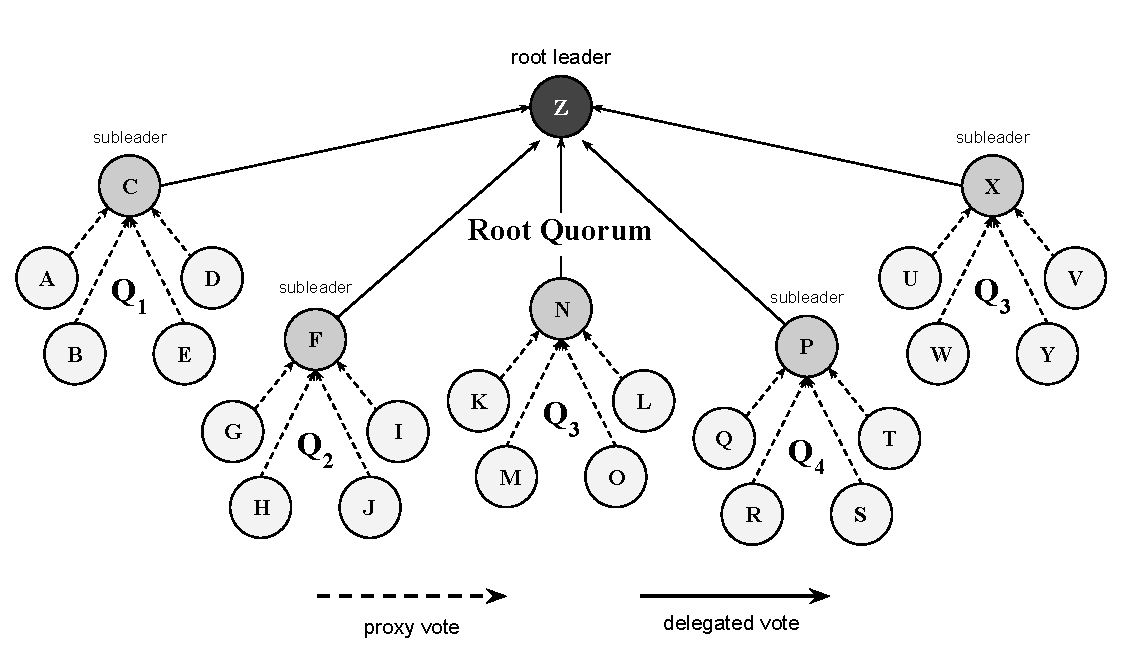
\includegraphics[width=0.5\textwidth]{figures/delegates}
\vspace{-.15in}
    \caption{Followers in subquorums guarantee
      intersection between the root and subquorums by delegating their votes to the subleader.}
    \label{fig:delegates}
\vspace{-.3in}
\end{figure}

\subsection{Operation}

The root consensus group coordinates all decision space changes.
% Consider the simple example of the transfer of object responsibility from one subquorum
% to another:
% 
% Pete: I'm not a fan of this notation, was just following from what I had above. I think
% we could probably go back to the ABC --> ABGH notation.
% \begin{quote}
% \small
%    $Q_1: \{o_a,o_b,o_c\} \rightarrowtail \{o_a,o_b,o_g,o_h\}$\\
%    $Q_2: \{o_d,o_e,o_f,o_g,o_h\} \rightarrowtail \{o_c,o_d,o_e,o_f\}$
% \end{quote}
For example, assume
each of two subquorums, $Q_1$ and $Q_2$, wants to give up a portion of its
existing decision space and to add objects currently mapped to another subquorum.
Reallocating subquorums requires a two phase consensus decision.
Both subquorum leaders send change requests to the leader of the parent quorum, which may
aggregate several requests into a single namespace change.
While the parent quorum gets consensus to make the epoch change, subquorums can continue
operating on their own decision space.
Once the parent quorum updates the epoch, it communicates the change to all affected
subquorums.
Each subquorum independently decides when to transition to the new epoch.
Subquorums in the new epoch can only access newly-gained objects once they have been
released by the objects' owners in the last epoch.

\subsection{Epochs and Ordering}

Hierarchical consensus requires all accesses in each subquorum to be linearizable,
guaranteed by serializing all accesses through the subquorum leader.
Global linearizability is guaranteed by serializing epochs at the parent
quorum, and limiting clients to access only one subquorum per epoch (relaxed
below).

Let \emph{interval} $i_e$ be the ordered set of accesses of the replicas in subquorum
$Q_i$ during epoch $e$.
We enforce linearizable ordering of all accesses in the entire system by
ensuring that there must exist a total ordering of the intervals that produces the correct
access results.
Access results should be equivalent to any interval ordering
such that all intervals in $e$ occur before intervals in $e+1$ (our ``interval
ordering'' invariant).
This is because there is no cross-traffic between any $Q_i$ and $Q_j$, and therefore
ordering interval $i_e$ before $j_e$ is exactly the same as ordering interval $j_e$
before $i_e$, for any $i$, $j$, and $e$.

The internal invariant requires $\forall_{x,y} : Q_{x,e} \rightarrow Q_{y,e+1}$.
Ordering all accesses according to consensus-based log order and interval order satisfies both the
internal invariant and linearizability  while still allowing subquorums to operate
independently within epochs.
Given $Q_i$ and $Q_j$ within epochs $e=1$ and $e=2$, one possible interval order is
$Q_{i,1} \rightarrow Q_{j,1} \rightarrow Q_{i,2} \rightarrow Q_{j,2}$.

% \subsubsection{Remote Accesses}
% \label{sec:remote}
\vspace{.03in}
\noindent
\textsl{Remote Accesses:}
By default we assume that the set of replicas \emph{assigned} to subquorums are also
disjoint, and that all accesses through a replica of a given subquorum are mapped to the
local decision space.
This is often reasonable.
However, if an object is assigned to a decision space and a replica in another subquorum
wishes to
access it, the system must either disallow the access (our default approach) or take
explicit notice that a dependency has been created between the subquorums.

The latter approach requires a serialization of all accesses currently within the remote
quorum with respect to all accesses before the remote access in the local quorum.
Assume a read access from $Q_k$ to $Q_i$ in epoch $e$; at the time of the read all
accesses in $Q_i$ must $\rightarrow$ all accesses following the read.
We accommodate this requirement by using the read endpoints to break interval $i_e$ into
$i_{e.1}$ and $i_{e.2}$ at the point $Q_i$ receives the remote access, and interval $k_e$
into $k_{e.1}$ and $k_{e.2}$ at the point $Q_k$ receives a response as shown in
Figure \ref{fig:fuzzy}.
Our results are consistent with total interval ordering by incorporating $Q_{i.1}
\rightarrow Q_{i.2}$.
Remote accesses are expensive and the runtime system must weigh the cost of repeated
remote accesses against the cost of epoch changes.

% \subsubsection{Fuzzy Epochs}
\vspace{.03in}
\noindent
\textsl{Fuzzy Epochs:}
Only subquorums involved in decision space changes need take notice of
epoch changes.
Other subquorums can move to a new epoch at no cost when informed of new epoch
numbers from remote requests.
Slow-responding subquorums therefore do not block decision space changes for other
quorums.
Safety is guaranteed because no writes in the next epoch depend on these writes.
These ``fuzzy epochs'' (Figure~\ref{fig:fuzzy}) allow an epoch change to be implemented solely by the
root quorum, allowing subquorums to move to the new epoch independently.
This flexibility is key to coping with partitions and varying connectivity in
the wide area.

\begin{figure}[t]
    \centering
    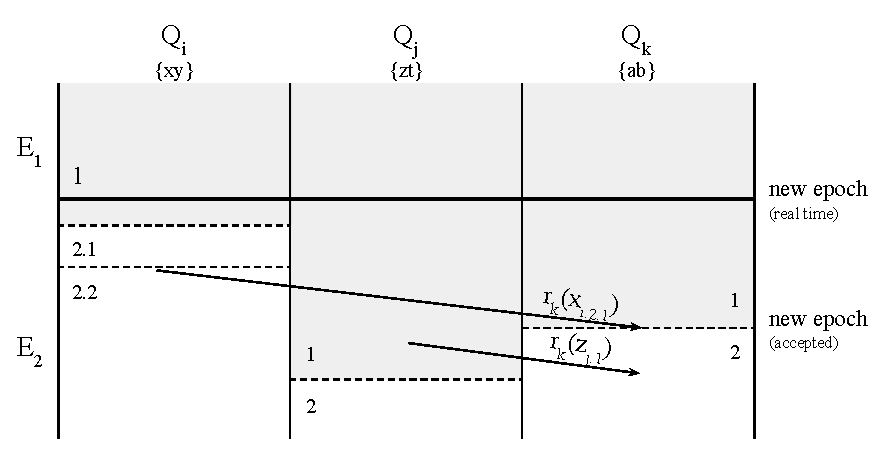
\includegraphics[width=0.5\textwidth]{figures/fuzzy}
    \caption{The gray region shows the ``fuzzy'' boundary between epochs $E_1$
      and $E_2$. $r_k(x_{2.1})$ reads the value of object $x$ from $Q_i$ into
      $Q_k$ and forces $Q_k$ to change epochs.}
    \label{fig:fuzzy}
\vspace{-.2in}
\end{figure}

% \subsubsection{Linearizability}
\vspace{.03in}
\noindent
\textsl{Linearizability:}
The primary goal of hierarchical consensus is strong consistency in the form of a
globally agreed upon linearizable ordering of read and update accesses.
By combining the internal ordering invariant and subintervals on remote access,
hierarchical consensus can be seen as defining the ordering of accesses in a grid
(Figure~\ref{fig:linearizability}).
If traditional consensus can be seen as assigning operations to positions in a log,
hierarchical consensus can be seen as assigning positions in a grid.
The root quorum partitions the grid into major rows (each epoch) and major columns
(each subquorum).
Subquorums assign positions to cells in the current row, while remote accesses create
new minor rows within each epoch.
Once constructed, a global ordering is achieved that is maintained by \emph{all} replicas,
who read the grid left to right, top to bottom.


\begin{figure}[t]
    \centering
    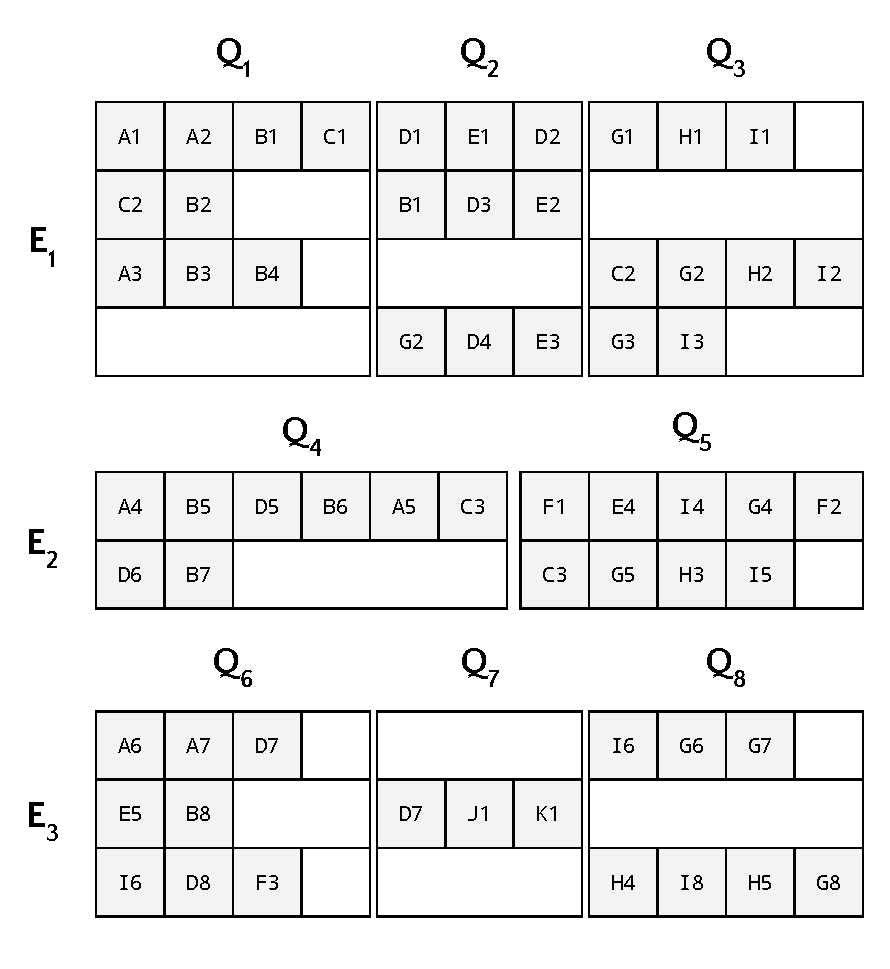
\includegraphics[width=0.4\textwidth]{figures/linearizability}
    \caption{Hierarchical consensus provides linearizability by ordering operations from left to right, top to bottom.}
    \label{fig:linearizability}
\vspace{-.2in}
\end{figure}


\section{Correctness Sketch}

We assert that consensus at the leaf nodes is correct and safe because decisions are
implemented using well-known leader-oriented consensus approaches.
Hierarchical consensus therefore has to demonstrate linearizable correctness and safety
between subquorums for a single epoch and between epochs.
Briefly, linearizability requires that external observers view operations to objects as
instantaneous events.
Within an epoch, the subquorum coordinates read and write accesses, and thus guarantees
linearizability for all replicas in that quorum.
Remote accesses and the internal invariant also enforce linearizability of accesses
between subquorums.
Epoch transitions raise the possibility of objects being re-assigned from one subquorum to
another, with each subquorum making the transition independently. Correctness is
guaranteed by an invariant that acquiring subquorums delay accessing newly acquired objects
until receiving notice that the releasing subquorum(s) have transitioned, \emph{plus} a
description of object versions at the point of this transition.


% \section{Experimental Design}
% 
% We propose to implement a distributed file system called FluidFS to more completely explore
% the use of hierarchical consensus in supporting file systems.
% FluidFS, implemented in the Go programming language, will allow us to quantitatively
% describe real-world environments and usage and to show how our proposed consistency
% model is experienced by users.
% 
% FluidFS will provide \emph{close-to-open consistency} (CTO), meaning that a file
% open, which implies a full-file read, is guaranteed to see the data written by the ``most recent'' close of
% that file.
% Therefore file opens and closes must be totally ordered, and map
% easily onto operations in a replicated log.
% The canonical use of CTO is a single-server case, where a total
% ordering of file open and closes is just the ordering that the opens
% and closes arrive at the server.
% The distributed case assumed by this work is much more demanding because
% opens and closes are distributed across servers throughout the system.
% 
% We leverage hierarchical consistency to build a distributed set of sequentially-consistent logs
% that guarantee a total ordering over all file accesses.
% The result is a similar user experience to having the user/client co-located with a single
% server, while the user migrates around the system, using different devices, possibly
% collaborating with other users, and tolerating network vagaries, partitions, and failures.
% 
% Note that FluidFS, like many modern file systems,
% decouples metadata file
% data storage~\emph{recipes}
% Metadata includes an ordered list of \emph{blobs}, which are opaque binary chunks.
% When a file is closed after editing, the data associated with the file is chunked into a
% series of variable-length blobs, identified by a hashing function applied to
% the data.
% The version created by the write access to the file specifies the blobs and their ordering
% that make up the file.
% Since blobs are effectively immutable, or tamper-evident, (blobs are named by hashes of
% their contents), we assert that consistent metadata replication can be decoupled from blob
% replication.
% Accesses to file system metadata becomes the operations or entries in the replicated logs.
% Metadata is therefore replicated through the system, allowing any file
% system client to have a complete view of the file system namespace.

\section{Discussion}

Hierarchical consensus flexibly allocates subquorums to dynamic object groupings.
Multiple subquorums means both more leaders and less global communication, reducing the
resource requirements for most nodes, preventing bottlenecks, and increasing throughput.
Consensus decisions can also be localized to where the accesses are occurring,
minimizing both distance and the effect of wide area network variability.
Finally, hierarchical consensus does not arbitrarily assign consensus decisions to single
objects or unrelated groups of objects, but to objects that are implicitly dependent on
each other because of their associated accesses.

% An open question for our research is how to automatically allocate the namespace such that
% leadership of a subset of the namespace is local to the accesses and that members of the
% quorum are distributed to provide wide area durability and availability.
% To explore this question as well as empirically show the scalability of hierarchical
% consensus, we are currently implementing a distributed file system called FluidFS.
% FluidFS will allow us to quantitatively describe real world environments and usage and
% to demonstrate how our proposed consistency model is experienced by users.

\bibliographystyle{ACM-Reference-Format}
\bibliography{paper}

\end{document}
